\chapter{界面粘接强度试验设计}
\section{研究现状和研究设计}
\subsection{电极活性层-集流体相关胶接作用研究}
基于之前对于锂离子电池电极内部结构(\ref{fig:structure})的介绍,进一步的说,无论是正极还是负极,除了活性颗粒之外内部还掺杂着导电剂和粘结剂,而后者在各个成分的粘接中发挥了至关重要的作用。 实际上,活性层和集流体之前的连接的建立也是依靠着内部的粘结剂而形成\cite{Haselrieder2015Measuring}。
在电极活性材料的制备和其涂布的过程中,由于活性层内部材料组成成分的多样、活性颗粒的形状大小不一等因素,以及粘结剂会和活性物质相互作用\cite{Liu2012Particles}而产生重新分布造成复杂的内部结构\cite{Lee2007A,Stevenson2008The},都使得对于活性层的力学特性的研究面临着相当大的困难\cite{Yoo2003Effect}。\\
\indent 总之,在电池的工作循环中,颗粒之间,颗粒和集流体之间的粘接强度对于保证电极的力学完整性乃至电化学功能有着十分重要的作用。 已经有研究表明,这一粘接强度对于电极的电流传导\cite{Chen2003Comparison}和电池的容量保持\cite{Lee2006Effect}都有着相当大的影响。 而更加重要的是,在前文已经指出,对于高容量的电池而言,其电极材料往往会由于可以容纳更多的Li离子从而会产生更大的体积变化,此时胶接强度就显得更加重要。因此,有必要对于电极的胶接强度特性进行完整的力学测试和建模,从而指导电极的设计和优化。 另外,对于电动汽车在碰撞事故过程的分析中,需要对电池包进行冲击工况的建模,此时界面的粘接强度的一系列力学参数都需要实验予以标定和整合。
\subsection{胶接作用影响因素}
活性层和集流体的粘接强度受着多种因素影响,由电极的内部结构所决定\cite{Seki2004Effect,Jing2008Effect},取决于电极中不同颗粒之间以及颗粒和集流体之前的物理吸附和化学键合的特性。 通常而言,粘接强度取决于活性物质之间的接触和粘接乃至活性物质和基底(即构成集流体的金属箔)之前的粘接,从而活性颗粒的尺寸大小颗粒之前形成的接触的种类和个数都主导着胶接强度的大小\cite{Kwade}。 而之前的研究已经从诸如其组成材料\cite{Yoo2003Effect,Chen2006Binder,Liu2005Enhanced}(活性颗粒、金属箔和粘接剂)之间的物理化学的界面相互作用、电极的组成结构\cite{Buqa2006Study,Liu2012Particles,Stevenson2008The}乃至电极的生产过程\cite{Lee2007A,Jing2008Effect,Park2007Mechanical}等不同尺度和角度展开。接下来将首先对于之前的研究胶接强度的研究进行简要综述,再介绍本文所设计和采用的研究方法。
\begin{figure}
\centering   
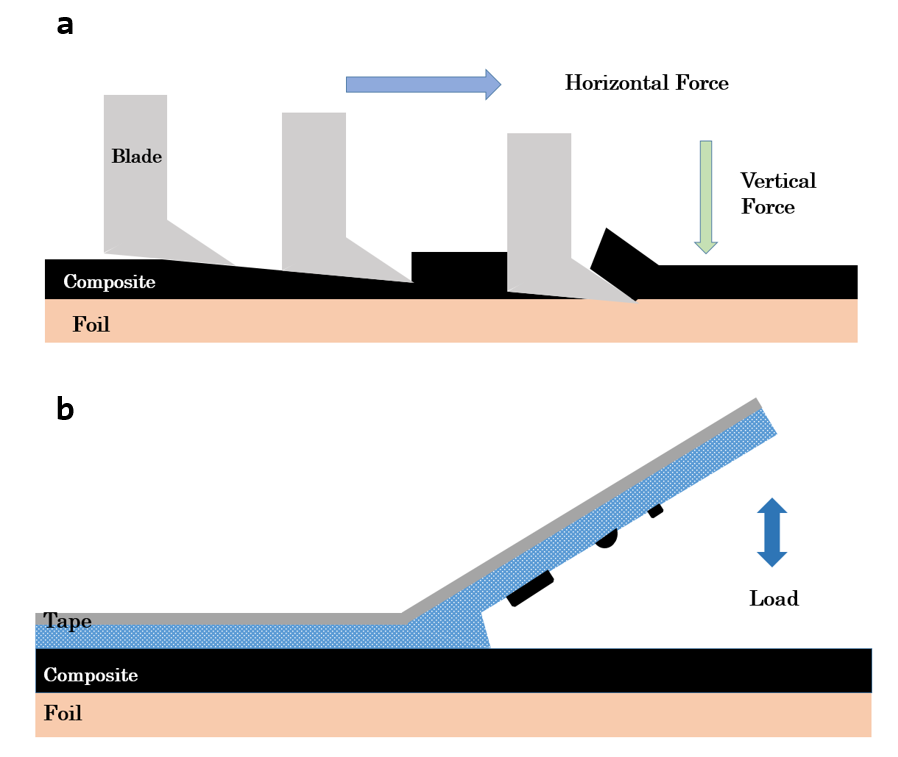
\includegraphics[width=\textwidth]{previoustest.png}
\caption{对活性层界面强度的测试方法:(a)SAICAS测试(纳米压痕法) (b)传统的Peel测试} 
\label{fig:pretest}
\end{figure}
\subsubsection{胶接强度试验方法调研}
之前的强度测试主要有两种方法,如图\ref{fig:pretest}所示。 Peel测试(见图\ref{fig:pretest}(a))实际上是使用胶带从集流体上利用黏性将活性物质粘离,从而得到测试界面强度的数据。由于该测试方法操作简便,能大致估算出界面强度,所以在工业界得到了广泛应用。比如之间有研究用这一方法来测量活性层和金属薄膜基底之前的粘结强度,并探究了诸如悬浮工艺(在负极生产中采用)对于电极强度的影响\cite{Park2011Effect}。 但是,这一操作相对简单的方法的测试结果十分受到诸如使用的胶带的种类,胶带和测试样品的起初的粘接强度等因素的影响。 另外,Peel测试中,几乎所有的断裂都发生在活性层的较浅的表层,所以其测得的粘接强度是表面的而不是整个体材料的,更不用说几乎无法测得活性层和集流体的粘接强度。 也就是说,通过Peel测试得到的粘接强度所对应的失效位置是难以确定的并且也无法得到活性层-集流体界面的粘接强度这一在建模中十分重要的参数。\\
\indent 另外一种方法是利用纳米压痕的方法测定给定深度和位置的粘接强度(SAICAS\cite{Son2014Measurement}),这一方法同时也可以用于对电极断裂的演变的研究\cite{Saito2010An}。 但是其测试结果很难被直接转化为活性层-集流体的粘接强度,而且并不能研究复杂加载乃至动态加载的力学响应行为。\\
\indent 接下来将介绍所设计的一种可以在混合拉伸-剪切工况下测量电极活性层-集流体粘接强度的测试方法,这一测试方法同时也可以很好的进行不同应变率加载的测试。 本章将首先介绍实验方法的详细设计和实验分析所会用到的断裂准则和材料模型,对于具体电极(包括正负极在不同角度加载实验和动态实验)的实验结果及其分析将在第三章详细说明。
\subsection{实验方法设计}
\subsubsection{试样设计}
在试验中,所研究的对象是活性层-集流体-活性层这样的三明治结构,即由两侧的多孔的活性物质粘附在中间的金属薄膜上构成。 考虑到整个电极的纵向厚度不超过200$\mu m$,所以很难对这一结构施加直接的边界约束从而展开力学测试。 所以在实验中,将活性层的两侧通过胶水粘附到两侧的基底上再对试样固定到夹具上进行实验,如图\ref{fig:specimen}所示。
\begin{figure}
\centering   
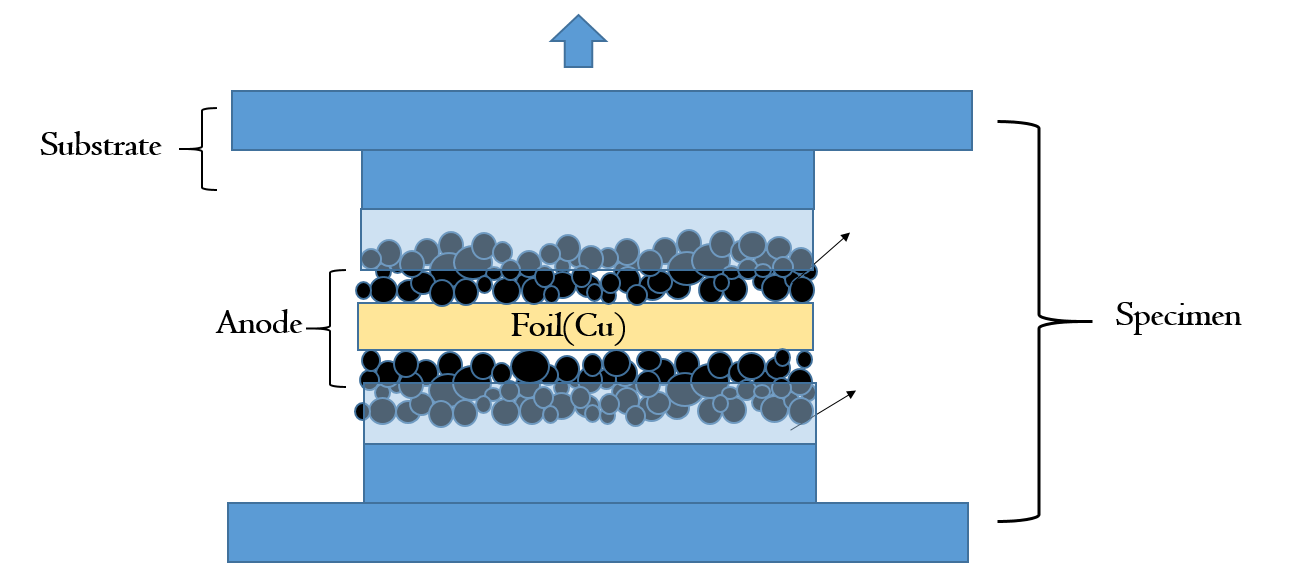
\includegraphics[width=\textwidth]{Specimen.png}
\caption{试样的结构示意图} 
\label{fig:specimen}
\end{figure}
\\
\indent 由于所研究的结构为一个多种物质构成的多层次结构,所以显而易见,在力学加载过程中,其可能发生的断裂失效模式有三种,如图\ref{fig:mode}所示。 失效分为,基底和活性层之间的断裂(这可以通过使用强度合适的胶水和改进涂布方法得到避免),活性层内部的断裂失效(这也称为内聚失效)和活性层和集流体之前的脱层失效(即粘接失效)。由于实验的测定目的为研究活性层和集流体之前的脱层失效,则希望力学测试中失效行为都为第三种失效,即断裂都发生在活性层和集流体之间。
\begin{figure}
\centering   
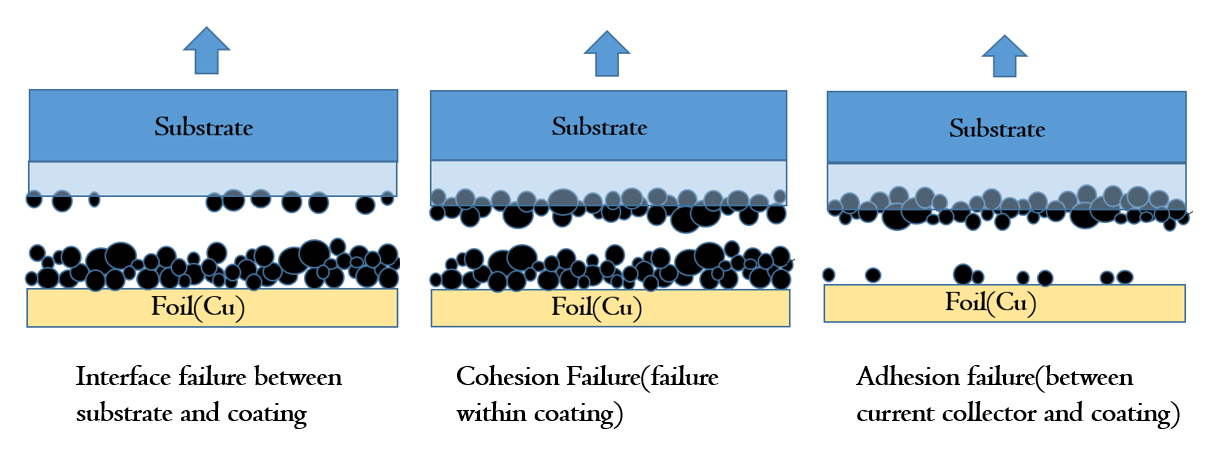
\includegraphics[width=\textwidth]{failuremode.png}
\caption{不同的断裂失效模式: 基底和活性层之间的断裂, 活性层内部的断裂和活性层和集流体之间的断裂} 
\label{fig:mode}
\end{figure}
\\
\indent 为了达成这一目的,将一侧用渗透性很强的胶水代替,从而能使得第一种断裂很难发生;另外,研究表明,由于活性层的涂布工艺,内部粘结剂的含量从外侧到集流体侧逐渐减小\cite{M2017Investigation},使得第二种失效相对第三种失效不易发生,从而只需要考虑另外一侧(即图中加载侧)的断裂。 而在实际的试验中,在下侧使用液体万能胶(Super Glue 15187)粘接,而上侧选用了特殊的凝胶(Loctite Super Glue)粘接,从而可以保证失效只在上侧发生并主要是第三种失效模态。(见图\ref{fig:geltype})。在液体胶侧,液体胶很容易整个渗透入活性层的多孔结构中,这会大大增强其力学强度并且这一侧的集流体-活性层界面也会被加强。 而另外一侧,凝胶由于其很差的渗透性只在表面的很少部分粘接(后续部分会有具体的实验测定),从而不会影响到起初的这一侧的集流体-活性层的粘接。 通过这样的试样处理和制备,只有凝胶侧的集流体-活性层的粘接强度相对最低,从而在力学加载中最容易发生失效,从而就可以得到起初所希望得到的失效模式。
\begin{figure}
\centering   
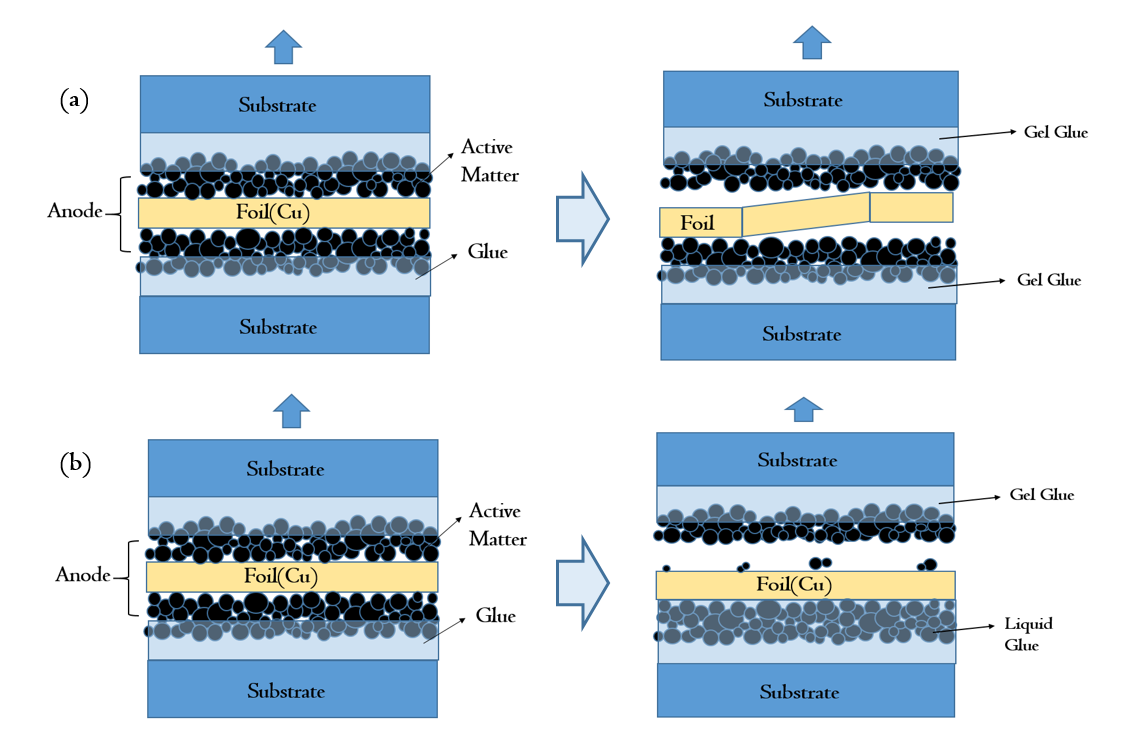
\includegraphics[width=\textwidth]{Geltype.png}
\caption{选用不同的胶水:(a)两侧选用凝胶使得可能发生图示失效 (b)一侧选用粘接性很强的液体胶从而使得只在凝胶侧发生失效} 
\label{fig:geltype}
\end{figure}
\subsubsection{混合拉伸-剪切实验设计}
\begin{figure}
\centering   
\includegraphics[width=\textwidth]{Combine.png}
\caption{混合拉伸-剪切实验设计:(a) 夹具和样品实物图 (b)混合测试示意图} 
\label{fig:combine}
\end{figure}
为了实现对于混合拉伸-剪切应力加载条件下的测试,设计了如图所示的实验夹具,如(b)所示,样品被粘接在两个基底上然后在固定在夹具上进行测试,夹具的加载方向实现了从$0^{\circ}$到$90^{\circ}$每隔$15^{\circ}$的一共七组加载条件的测试。 显然随着角度的增加,剪切分量增加。 静态实验的测试设备如图\ref{fig:equipment}所示,采用的静态测试速度为$1.0mm \times min^{-1}$,每个实验至少重复三次。 动态实验的测试则如图\ref{fig:dynamic}所示,可以实现中低速的动态加载和力学测试。
\begin{figure}
\centering   
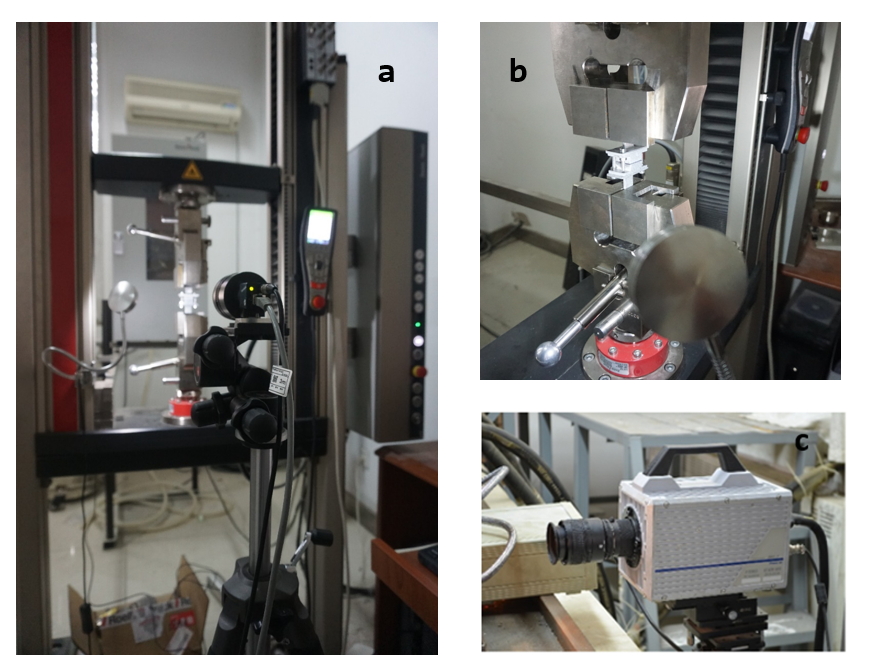
\includegraphics[width=\textwidth]{equip.png}
\caption{静态测试设备:(a)Zwick Z020 universal mechanical tester
(b) Tester with specimen (c)Digital image correlation(DIC) camera} 
\label{fig:equipment}
\end{figure}
\begin{figure}
\centering   
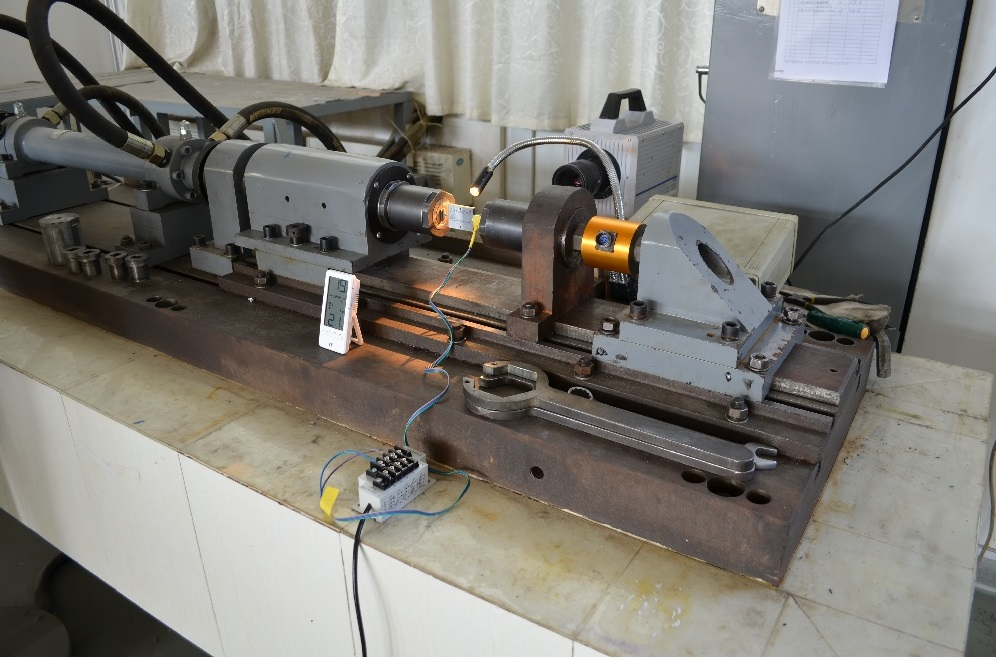
\includegraphics[width=\textwidth]{dynamic.png}
\caption{动态测试设备:液压加载水平台} 
\label{fig:dynamic}
\end{figure}
\section{实验准备和模型分析}
\subsection{测试样品分析:能谱测试}
正如之前所提到,实验成功的关键在于实现只在一侧发生活性层-集流体的脱层失效,之前的设计已经可以从原理上保证这一失效行为,但是还需要保证在发生断裂的这一侧,所涂布的凝胶不会有很强的渗透从而不会在断裂面上有凝胶的存在,从而不会对界面强度测试的结果产生影响。 基于此,对涂布的样品进行了沿着纵切面的电子能谱(Energy Dispersive Spectrdmeter,EDS)测试,其原理为,由于电极活性层中不含有硅元素,而所使用的特种凝胶中含有硅元素,所以通过测定硅元素在纵切面沿着深度的分布得到凝胶的渗透情况,测试结果如图\ref{fig:eds}所示。从图中可以看出,硅元素的分布只在很浅的表层,从而凝胶的渗透只在很浅的深度,不会影响到发生在活性层和集流体之间的断裂失效。
\begin{figure}
\centering   
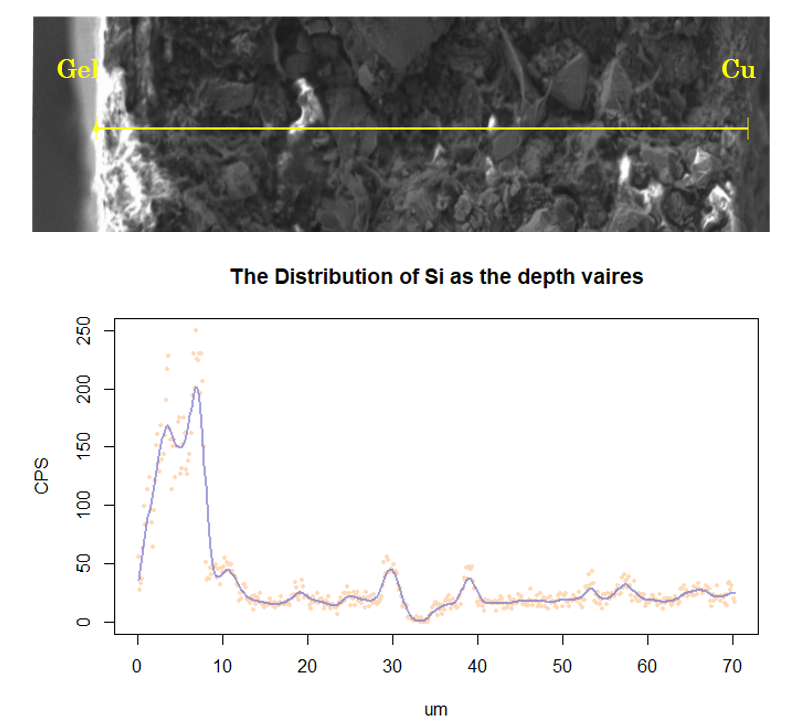
\includegraphics[width=\textwidth]{EDS.png}
\caption{沿着深度方向从涂胶侧到集流体侧的硅元素丰度的分布} 
\label{fig:eds}
\end{figure}
\subsection{断裂准则}
在本文所进行的活性层-集流体断裂失效行为的研究中,其中最为关键的是得到力学加载时的峰值力,也就是断裂失效对应的断裂强度。 之所以研究不同方向的加载以产生混合拉伸-剪切的实验加载条件,是为了准确表征界面断裂失效行为,从而对其进行表征从而预测其在各种混合工况下的失效行为。对于材料的断裂失效进行研究,最核心的便是研究清楚其屈服面以及对应可以采用的屈服准则,所以有必要首先对于材料的屈服特性乃至主要的屈服准则进行一个概要的介绍。
\subsubsection{屈服面}
通常而言,材料的屈服面是一个五维平面(六维应力空间中),其通常为凸集且在屈服面内材料处于弹性状态。 之所以叫做屈服面,也就是当材料的应力状态到达屈服面上一点(也就是其屈服点),材料就进入了塑性状态,并且进一步的加载只是会使得材料继续在该屈服面上移动,改变其应力状态\cite{Hughes}。\\
\indent 依据这样的假定,有许多针对具体材料特性和基于实验观测的屈服准则被提出。 
一般而言,屈服准则都被表达为三个主应力($\sigma_1,\sigma_2,\sigma_3$)或者应力的三个不变量($\mathbf{I_1},\mathbf{J_2},\mathbf{J_3}$)的函数形式\cite{Hughes}:
\begin{equation}
\mathnormal{f}(\sigma_1,\sigma_2,\sigma_3) = 0
\end{equation}
或者
\begin{equation}
\mathnormal{f}(\mathbf{I_1},\mathbf{J_2},\mathbf{J_3}) = 0
\end{equation}
需要指出的是,对于三个主应力,可以得出应力的三个不变量和它们的关系:
\begin{equation}
I_1 = \mathrm{Tr}(\mathbf{\sigma}) = \sigma_1 + \sigma_2 + \sigma_3
\end{equation}
\begin{equation}
J_2 = \frac{1}{2} \mathbf{s} : \mathbf{s} = \frac{1}{6} \left[(\sigma_1-\sigma_2)^2 + (\sigma_2-\sigma_3)^2 + (\sigma_3-\sigma_1)^2 \right]
\end{equation}
\begin{equation}
J_3 =det(\mathbf{s}) = \frac{1}{3}(\mathbf{s} \times \mathbf{s}) : \mathbf{s} =s_1s_2s_3
\end{equation}
其中,
\begin{equation}
s = \sigma - \frac{I_1}{3}\mathbf{I} 
\end{equation}
\subsubsection{主要屈服准则}
\begin{figure}
\centering   
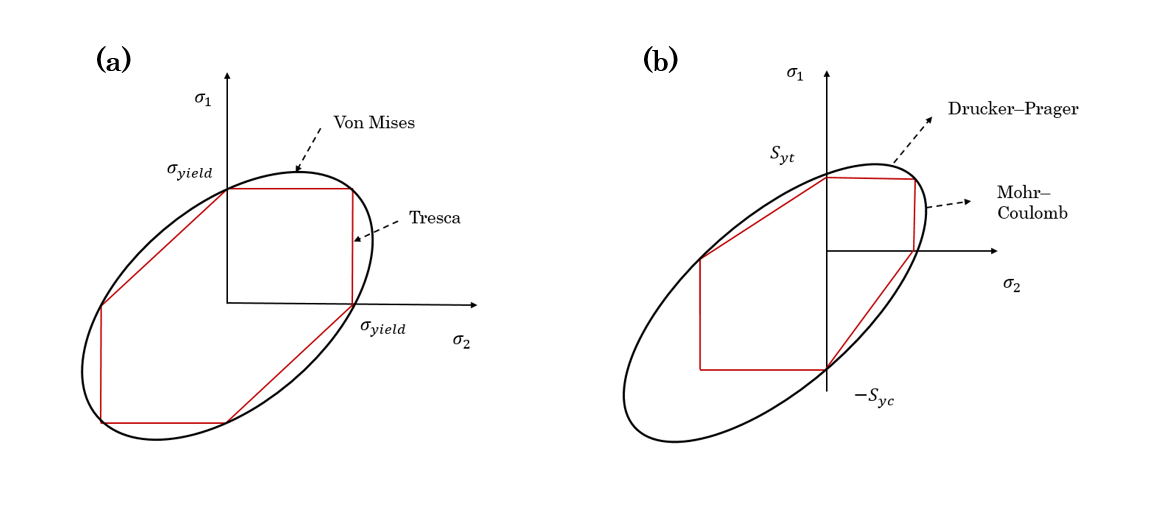
\includegraphics[width=\textwidth]{yield.png}
\caption{(a)Von Mises和Tresca失效准则 (b)Drucker-Prager和Mohr-Coulomb失效准则} 
\label{fig:yield}
\end{figure}
工程中常用的屈服准则有一下几种\cite{Jagab2005Theory}:
\begin{itemize}
	\item Tresca 失效准则\\
	Tresca失效准则又称最大切应力准则(Maximum shear stress theory),其数学表达为:
	\begin{equation}
	\frac{1}{2}\left(|\sigma_1-\sigma_2|,|\sigma_2-\sigma_3|,|\sigma_3-\sigma_1|\right)=S_{sy}=\frac{1}{2}S_y
	\end{equation}
	其中,$S_{sy}$是剪切失效强度而$S_y$是拉伸失效强度。主应力空间中Tresa屈服面是一个六边的菱形,其在受到静水压力(三个主应力大致相等)时材料一直保持弹性,而当主应力有不一致时,材料会受到剪切,若剪切到达屈服水平材料进入塑性。图\ref{fig:yield}(a)展示了二维应力空间的屈服面。
	\item von Mises 失效准则\\
	von Mises失效准则的数学表达为:
	\begin{equation}
	(\sigma_1 - \sigma_2)^2 + (\sigma_2 -\sigma_3)^2 + (\sigma_3-\sigma_1)^2 = 2S^2_y
	\end{equation}
	其中,$S_y$是拉伸失效强度。其失效面是一个圆柱体,轴向和三个主应力方向夹角相同,其在二维应力空间的屈服面呈现椭圆形,如图\ref{fig:yield}(a)所示。
	\item Mohr–Coulomb 失效准则\\
	Mohr-Coulomb准则和Tresca失效准则相似,只是考虑了材料的拉伸和压缩模量不同的情况,所以通常在表征土壤、混凝土等颗粒状材料的断裂中有很广泛的应用。其数学表达式为:
	\begin{multline}
	\frac{m+1}{2} \mathbf{max} \Big(|\sigma_1 - \sigma_2| + K(\sigma_1+\sigma_2),|\sigma_1 - \sigma_3| + K(\sigma_1+\sigma_3),|\sigma_2 - \sigma_3| + \\
	K(\sigma_2+\sigma_3)\Big) = S_{yc}
	\end{multline}  
	其中
	\begin{equation}
	m = \frac{S_{yc}}{S_{yt}}
 \quad K=\frac{m-1}{m+1}
 	\end{equation}
 	参数$S_{yc}$和$S_{yt}$分别是材料的压缩和拉伸失效强度,显然当材料的拉伸和压缩参数相同,即$S_{yc}=S_{yt}$时,该准则就会退化为Tresca准则。
 	图\ref{fig:yield}(b)展示了其在二维应力空间中的失效面。
	\item Drucker–Prager 失效准则\\
	和von Mises失效准则类似,该准则用于处理拉伸和剪切都可能引起断裂失效的情况,如对混凝土材料,其数学表达式如下:
	\begin{multline}
	\left(\frac{m-1}{2}\right)(\sigma_1 + \sigma_2 + \sigma_3 )+\left(\frac{m+1}{2}\right)
	\sqrt{\frac{(\sigma_1-\sigma_2)^2+(\sigma_2-\sigma_3)^2+(\sigma_3-\sigma_1)^2}{2}}\\
	=S_{yc}
	\end{multline}  
	其中
	\begin{equation}
	m = \frac{S_{yc}}{S_{yt}}
	\end{equation}
	其在二维应力空间的图线如图\ref{fig:yield}(b)所示。
\end{itemize}

\subsection{胶粘失效模型——内聚力模型}
对于大多数的断裂问题,诸如已经存在裂纹和裂纹前的应力奇异区域可以忽略的情况,应用线弹性断裂力学的工具就可以分析得到足够好的结果。但是对于韧性较大的材料和或者
粉体类材料,由于其塑性行为和微裂纹的影响,其发生断裂时裂纹尖端的非线性区不能被忽略。 而在这些情况下,由 Hillerborg 所提出的内聚力模型\cite{Hillerborg2008Analysis},便成为解决这些问题的重要工具。\\
\indent 特别地,对于复合材料而言,多种材料之间的脱层失效是诸如纤维增强材料断裂失效的主要模式。 脱层失效还可以在多种情形下发生,即使在低速甚至静态的外载,在结构点的受力都有可能引起脱层失效\cite{Elices2002The}。 由于脱层失效实际上很难被发现,所以对于其模式的研究和表征就显得十分重要。 对于这样的问题,内聚力模型提供了十分重要的工具。\\
\indent界面的脱层失效的断裂问题归根结底是不连续性的问题。 考察包含不连续(发生了断裂或者脱层)的区域$\Omega$,而$\Gamma_d$将区域$\Omega$划分为两部分,$\Omega_{+}$和$\Omega_{-}$。而在边界$\Gamma_{F}$上有预先给定的外力。 则可以用一下方程描述区域内的应力$\sigma_{ij}$(用$\sigma^{+}_j$和$\sigma^{-}_j$表示不连续的应力)\cite{Turon2007An}:
\begin{equation}
\sigma_{ij,j} = 0 \quad in \quad \Omega
\end{equation}
\begin{equation}
\sigma_{ij}n_j = t_i  \quad on \quad \Gamma_F
\end{equation}
\begin{equation}
\sigma_{ij} n^{+}_j = \tau^{+}-i = -\tau^{-}_i = \sigma_{ij}n^{-}_j \quad on \quad \Gamma_d
\end{equation}
\indent 内聚力模型假定在断裂区产生一个粘接损伤带(Cohesive damage zone),从而可以将微结构的失效和连续力学场建立联系。 后文将利用这一模型的一个引申结论表征不同角度加载活性层的断裂失效强度。 \\
\indent 内聚力模型相比经典的断裂力学(线弹性断裂力学,裂纹尖端张开位移法)有着下列主要的优点:
\begin{itemize}
	\item 可以相对准确地预测材料的断裂失效
	\item 在分析中非线性区域不需要被忽略
\end{itemize}
实际上,内聚力模型本身并不基于任何材料模型,其本质上只是对材料之间被拉开时对于其间的粘接力的一个描述。 当粘性表面发生分离时,牵引力增加,直到达到最大值,然后随后减小到零,最终导致完全分离。 将牵引力-位移曲线绘制出便得到了牵引-位移曲线,同时该曲线下和坐标轴所围成的面积和分离所消耗的能量相等。 可以看出内聚力模型保持着连续性条件,在实现了物理上的分离的同时消除了应力的奇异度。更具体而言,内聚力模型所给出的牵引-位移曲线相当于给定了材料的断裂本构。\\
\indent 首先本文给出了内聚力模型的示意图\ref{fig:crack}(a)和其经典的牵引-分离曲线\ref{fig:crack}(b)。
\begin{figure}
\centering   
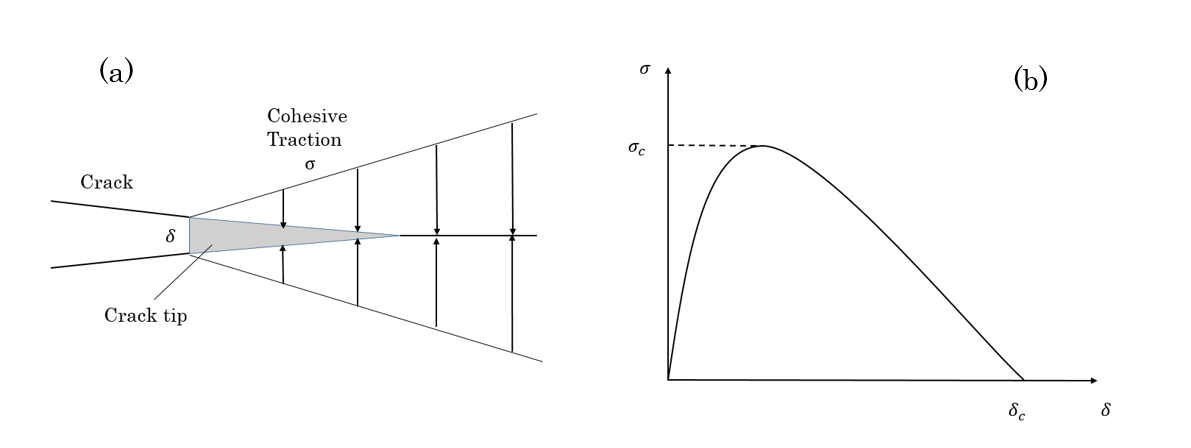
\includegraphics[width=\textwidth]{crack.png}
\caption{(a)内聚力模型示意图 (b)典型的牵引-分离曲线} 
\label{fig:crack}
\end{figure}
一般地,可以用下式来描述内聚模型中的牵引-分离关系
\begin{equation}
\sigma = \sigma_c \mathnormal{f}(\delta / \delta_c)
\end{equation}
其中,$\delta_c$是分离力的峰值,而$\sigma_c$是分离的特征位移。其无量纲的分离函数$\mathnormal{f}$和失效机理相关。\\
同时也可以求出粘接能量密度,也就是分离单位面积所需要做的功:
\begin{equation}
\Gamma_c = \int^{\delta_c}_0 \sigma(\delta) d\delta
\end{equation}
也就是曲线和坐标轴所围成的面积。下面将介绍一些对于函数$\mathnormal{f}$的一定程度的简化求解方法\cite{Elices2002The}:
\begin{enumerate}
	\item Dugdale 模型\\
	对韧性材料而言,其带状塑性区就是粘性区域,而屈服应力就是牵引力,如图\ref{fig:czm}(a)所示:
	\begin{equation}
	\sigma = \sigma_c
	\end{equation}
	同时有
	\begin{equation}
	\Gamma_c = \sigma_c\delta_c
	\end{equation}
	在使用这一模型时,完全分离在$\delta = \delta_c$时发生。
	\item 线性软化模型\\
	这一模型通常被用于模拟诸如陶瓷和混凝土这样的准脆性材料。其牵引-分离准则如下:
	\begin{equation}
	\sigma = \sigma_c(1-\delta/\delta_c)
	\end{equation}
	同时有
	\begin{equation}
	\Gamma_c = \frac{1}{2} \sigma_c \delta_c
	\end{equation}
	如图\ref{fig:czm}(b)所示,牵引力首先达到最值$\sigma_c$,然后随着分离位移增加而减小,最终在分离点$\delta_c$等于零。
	\item 梯形模型
	显然梯形模型\ref{fig:czm}(c)可以看成是上面的线性软化模型的一种延伸,其牵引-分离关系如下:
	\begin{equation}
	\sigma = 
	\begin{cases}
	\sigma_c(\delta/\delta_1)&\text{$0 \leq 
	\delta \leq \delta_1$}\\
	\sigma_c&\text{$\delta_1 \leq \delta \leq \delta_2$}\\
	\sigma_c(\delta_c-\delta)(\delta_c-\delta_2)&\text{$\delta_2 \leq \delta \leq \delta_c$}
	\end{cases}
	\end{equation}
	同时有
	\begin{equation}
	\Gamma_c = \frac{1}{2} \sigma_c (\sigma_c + \sigma_2 - \sigma_1)
	\end{equation}
	\item 指数模型\\
	基于原子尺度的模拟\cite{Rose1981Universal},可以建立指数形式的模型\ref{fig:czm}(d):
	\begin{equation}
	\sigma = \sigma_c \left(\frac{\delta}{\delta_0}\right)exp\left(1-\frac{\delta}{\delta_0}\right)
	\end{equation}
	其中,$\delta_0$是达到峰值牵引力$\sigma_c$时的分离位移,同时可以给出能量的计算公式:
	\begin{equation}
	\Gamma_c = \int^{\infty}_0 \sigma d\delta = \mathnormal{e} \sigma_c \delta_0
	\end{equation}
\end{enumerate}
\begin{figure}
\centering   
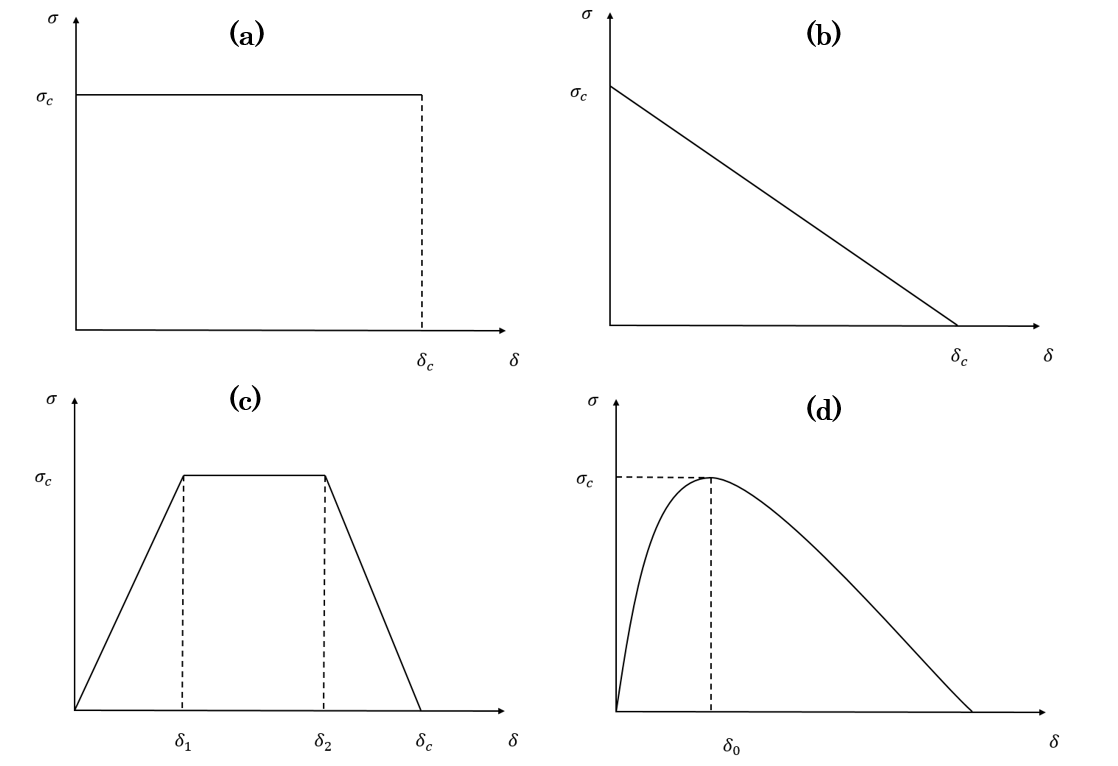
\includegraphics[width=\textwidth]{czm.png}
\caption{内聚力模型: (a)Dugdale 模型 (b) 线性软化模型 (c)梯形模型 (d)指数模型} 
\label{fig:czm}
\end{figure}
